\chapter{Fundamentals} \label{chap:fundamentals}
For much of human history, productivity growth was barely perceptible, and living standards improved at a snail's pace. Then approximately 200 years ago, a steep change in innovation occurred: the \textit{Industrial Revolution} treated as \textit{Industry 1.0}, in which the muscle power of all living beings was replaced by mechanical power that introduced steam engines and internal combustion engines to the mechanical production facilities. From the early part of the twentieth century, electrification and the division of labor led to the second industrial revolution which is referred as \textit{Industry 2.0} now. The third industrial revolution referred as \textit{Industry 3.0}, also known as the \textit{Digital Revolution}, was set in around the 1970s, when advanced electronics and Information Technology (\acs{IT}) developed further the automation of production processes. In the following decades industrial technological advancements were only incremental, especially compared with the breakthroughs that transformed \acs{IT}, mobile communications, and e-commerce \cite{INDUSINTERNET,IN4DESIGN,IN4BCG}.

Productivity and economic growth accelerated sharply in consequence of these innovations. The number of manufacturing jobs decreased, new jobs emerged and the demand for new skills grew. Today, another workforce transformation is on the horizon as manufacturing experiences a new wave of technological advancement where it is possible to augment physical machines with digital intelligence. The conditions are ripe and early evidence suggests that this new wave of innovation is already upon us \cite{INDUSINTERNET,MANMACHINE}.

In the next few sections, we have discussed about how the next industrial revolution will unfold itself, and its benefits for businesses and more broadly for economies around the world.
\section{Industry 4.0} \label{ind4}
The term \textit{“Industry 4.0”} that refers to the next industrial revolution became publicly known in 2011 at Hanover Fair, when an initiative named \textit{“Industrie 4.0”} - an association of representatives from business, politics, and academia - promoted the idea as an approach to strengthening the competitiveness of the German manufacturing industry \cite{VDINACH}. The German Federal Government supported the idea by announcing that Industry 4.0 will be an integral part of its “High-Tech Strategy 2020 for Germany” initiative, aiming at technological innovation leadership. The subsequently formed “Industrie 4.0 Working Group” then developed first recommendations for implementation, which were published in April 2013 \cite{IN4DESIGN}.

Hermann et al. \cite{IN4DESIGN} describe the fascination behind Industry 4.0 in 2 segments. Firstly, for the first time an industrial revolution is predicted a-priori, not observed ex-post that provides various opportunities for companies and research institutes to actively shape the future. Secondly, Industry 4.0 promises substantially increased operational effectiveness as well as the development of entirely new business models, services and products.
\subsection{Definition}
From the literature review of Hermann et al. \cite{IN4DESIGN} and Kagermann et al. \cite{VDINACH},
\begin{definition}
\textit{Industry 4.0} is a collective term for contemporary automation, data exchange, and manufacturing technologies and concepts of value chain organization which draws together Cyber-Physical Systems (\acs{CPS}), the Internet of Things (\acs{IoT}), Smart Factories and the Internet of Services.\footnote{\acs{CPS}, \acs{IoT}, \acs{IoS} and Smart Factory are the components of Industry 4.0. They are discussed later in \refsection{compoind4}.}
\end{definition}
Rüßmann et al. \cite{IN4BCG} explain it in a similar way as mentioned below.
\begin{definition}
\textit{Industry 4.0} is a new digital industrial technology that will connect sensors, machines, work-pieces, and \acs{IT} systems along the value chain beyond the enterprise which in turn will interact with another using standard Internet-based protocols and adapt to changes.
\end{definition}
In North America, similar ideas have been brought up under the name \textit{Industrial Internet} by General Electric \cite{INDUSINTERNET}. The technical basis is very similar to Industry 4.0, but the application is broader than industrial production. The various definitions have caused confusion rather than increasing transparency \cite{IN4HYPE}. Hereafter Industrie 4.0 or Industrial Internet or Integrated Industry will be referred interchangeably with Industry 4.0.
\subsection{Enablers of Industry 4.0}
\begin{figure}[h!]
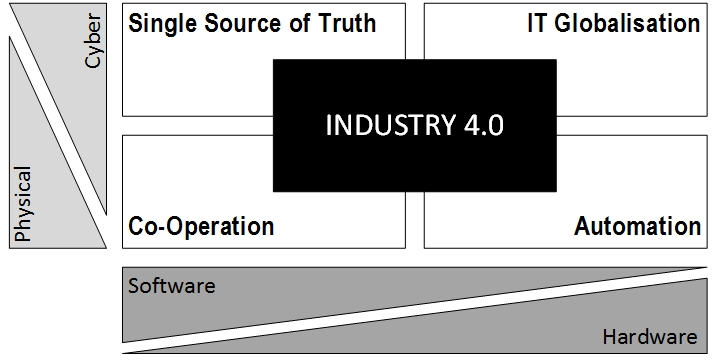
\includegraphics[scale=0.6]{./gfx/indus4enablers}
\centering
\caption{Four Enablers of Industry 4.0 - Adapted from \cite{IN4HYPO}}
\label{fig:2.1}
\end{figure}
Industry 4.0 is not initiated on a shop-floor level and therefore companies have to take measures in their own hands to introduce its enablers into their companies to profit from the current change in society and technology \cite{VDINACH}. 
These measures can be categorized by the aid of 2 dimensions. The first dimension describes whether a precondition is physical or cyber, whereas the second dimension allocates the precondition to hard- or software components. Industry 4.0 can be seen as a collaborated production by the inter-working of human-human, machine-human, and machine and production system as shown in \reffig{fig:2.1} \cite{IN4HYPO}.
\begin{itemize}
\item \textit{Single Source of Truth} dictates to embed all product life-cycle data along the value chain within a single database using cloud storage and accesses to make all changes to product and production visible and avoid ambiguity during production and simulations \cite{IN4HYPO}.
\item \textit{\acs{IT}-Globalisation} made computers achieve exponential growth in speed and cheap storage capacity. This will allow faster extensive simulations of different aspects of a company as well as the processing of huge amounts of data, which are already collected by companies, but cannot be used adequately \cite{IN4HYPO}.
\item \textit{Automation} leads to automated and decentralized processes which can be combined to collaboration networks and are able to adapt to dynamic requirements and therefore are self-optimizing \cite{IN4HYPO}.
\item \textit{Co-Operation} aims at the connection of all technologies and activities e.g. efficient sharing and exchange of engineering data within a network of engineers. Networks help to improve cooperation by communicating targets and empowering decision maker’s in decentralized systems \cite{IN4HYPO,VDINACH}.
\end{itemize}
\subsection{Components of Industry 4.0} \label{compoind4}
Advances in technology that powered Industry 4.0 are already used in manufacturing, but with Industry 4.0, they will transform production: isolated cells will come together as a fully integrated, automated, and optimized production flow, leading to greater efficiencies and changing traditional production relationships among suppliers, producers, and customers — as well as between human and machine \cite{IN4BCG}. Major factors that propels this next industrial revolution has been listed below.
\begin{itemize}
\item \textit{Cyber Physical Systems (\acs{CPS})} \footnote{\acs{CPS} is explained with its architecture in \refsection{CPS}.} are integrations of computation, networking and physical processes. Embedded computers and networks monitor and control the physical processes, with feedback loops where such processes affect computations and vice versa e.g. autonomous automotive systems \cite{IN4DESIGN}.
\item \textit{Internet of Things (\acs{IoT})} \footnote{\acs{IoT} is the prime driver of Industry 4.0 which is discussed in \refsection{IOT}.} allows field devices to communicate and interact both with one another and with more centralized controllers, as necessary. It also decentralizes analytics and decision making, enabling real-time responses \cite{IN4BCG,IN4DESIGN}.
\item \textit{Smart Factory} \footnote{Smart factory which thrives upon \acs{IoT} is discussed in \refsection{smartfactory}.} is context-aware by assisting people and machines in execution of their tasks. It is achieved by systems working in background, so-called Calm-systems and context aware means that the system can take into consideration information coming 	from physical and virtual world like the position and status of an object \cite{IN4DESIGN}.
\item \textit{Internet of Services (\acs{IoS})} enables service vendors to offer their services via the internet. The \acs{IoS} consists of participants, an infrastructure for services, business models, and the services themselves. Services are offered and combined as value-added services by various suppliers; they are communicated to users as well as consumers and are accessed by them via various channels \cite{IN4DESIGN}.
\item \textit{Big Data and Analytics} based on large data sets has emerged only recently in the manufacturing world, where it optimizes production quality, saves energy, and improves equipment service. Big data is high volume, high velocity, and/or high variety information assets that require new forms of processing to enable enhanced decision making, insight discovery and process optimization \cite{BIGDATA}. In an Industry 4.0 context, the collection and comprehensive evaluation of data from many different sources - production equipment and systems as well as enterprise- and customer-management systems - will become standard to support real-time decision making \cite{IN4BCG,IN4DESIGN}.
\item \textit{Cloud Computing} is a model for enabling ubiquitous, convenient, on-demand network access to a shared pool of configurable computing resources (e.g. networks, servers, storage, applications, and services) that can be rapidly provisioned and released with minimal management effort or service provider interaction as per definition of \acs{NIST} \cite{MELLNIST}. It will make increased data sharing across sites and company boundaries possible for Industry 4.0. At the same time, the performance of cloud technologies will improve, achieving reaction times of just several milliseconds. As a result, machine data and functionality will increasingly be deployed to the cloud, enabling more data-driven services for production systems \cite{IN4BCG,IN4DESIGN}.
\item \textit{Augmented Reality} based systems support a variety of services, such as selecting parts in a warehouse and sending repair instructions over mobile devices. These systems are currently in their infancy, but in the future, companies will make much broader use of augmented reality to provide workers with real-time information to improve decision making and work procedures \cite{IN4BCG}.
\end{itemize}
\subsection{Mechanisms to Increase Productivity}
The significant increase of the productivity due to Industry 4.0 can be represented by the 4 mechanisms. Schuh et al. \cite{IN4HYPO} discussed in their article how enablers of Industry 4.0 facilitate these mechanisms.
\begin{itemize}
\item \textit{Revolutionary Product Life-cycles}: Integrated technologies
and rapid prototyping facilitate companies to produce testable prototypes which supply viable information of the products potentials as customer feedback can be implemented immediately. Due to the new developments in \acs{ICT} the costs of an iteration and the resulting changes are not as cost intensive as before and therefore lead to a new development process in terms of time and profit which can be seen in \reffig{fig:2.2} \cite{IN4HYPO}.
\begin{figure}[h!]
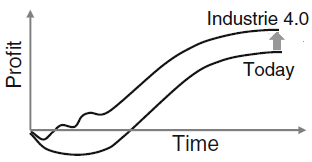
\includegraphics[scale=0.5]{./gfx/revlifecycle}
\centering
\caption{Industry 4.0: Revolutionary Product Life-cycles \cite{IN4HYPO}}
\label{fig:2.2}
\end{figure}
\item \textit{Virtual Engineering of Complete Value Chains}: By the aid of Software tools companies now have the opportunity to simulate their whole production network. This virtualization and simulation can reveal possible capacity problems as well as problems within the general workflow. By simulating the value chain in a short amount of time one is able to counteract possible problems before they arise, which enhances the decision capability which can be seen in \reffig{fig:2.3}. To get a valuable decision capability based on simulations	it is necessary to execute an adequate number of simulations \cite{IN4HYPO}.
\begin{figure}[h!]
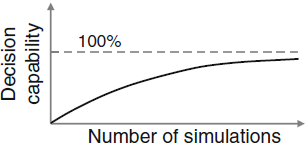
\includegraphics[scale=0.5]{./gfx/revsimul}
\centering
\caption{Industry 4.0: Virtual Engineering of Complete Value Chains \cite{IN4HYPO}}
\label{fig:2.3}
\end{figure}
\item \textit{Revolutionary Short Value Chains}: Companies have to offer more and more individualized products in order to meet the customer requirements. This complicates the division of labor introduced by Taylorism as machines in general are only able to accomplish one specific task. In order to allow even more individualized products the integration of production steps and thus the integration of functions within production systems is inevitable. This leads to a reversion of Taylorism - instead of the division of labor by means	of a conveyor belt production cells are to be established, allowing an employee to take over autonomous responsibility and give this specific employee decision \cite{IN4HYPO}. 

\begin{figure}[h!]
	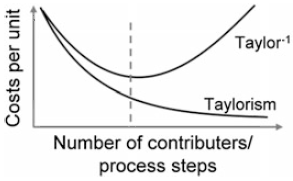
\includegraphics[scale=0.5]{./gfx/revvalchain}
	\centering
	\caption{Industry 4.0: Revolutionary Short Value Chains \cite{IN4HYPO}}
	\label{fig:2.4}
\end{figure}

Within a production process for highly customized products there is an optimal number of contributors or process steps in one production cell which have to collaborate in order to achieve minimal costs for the produced product which can be seen in \reffig{fig:2.4} \cite{IN4HYPO}.

\item \textit{Better Performing than Engineered}: Companies must aim at the self-optimizing	capabilities of production systems which are already theoretically possible. With the ongoing advancement of self-optimizing production systems machines should be able to reach a productivity level which exceeds the previously determined maximum due to cybernetic effects as shown in \reffig{fig:2.5}. An example would be a productivity of 15,000 units whereas the estimated maximum before self-optimization was 10,000 units \cite{IN4HYPO}.
\begin{figure}[h!]
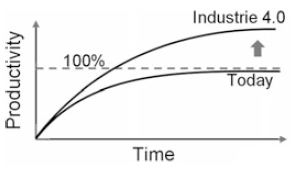
\includegraphics[scale=0.5]{./gfx/revengg}
\centering
\caption{Industry 4.0: Better Performing than Engineered \cite{IN4HYPO}}
\label{fig:2.5}
\end{figure}
\end{itemize}
\subsection{Industrial Requirements}
For Industry 4.0, the term revolution does not refer to the technical realization but to the ability to meet today’s as well as future challenges. Some very basic requirements guide most of the work currently being done.
\begin{itemize}
\item \textit{Investment Protection}: Industry 4.0 has to be introduced stepwise into existing plants with-out hampering business and investor's trust \cite{IN4HYPE,IN4BCG}.
\item \textit{Stability}: Industry 4.0 must provide stability and must not compromise production, neither by disturbances nor by a breakdown \cite{IN4HYPE}.
\item \textit{Infrastructure Development}: Industry 4.0 will require an	adequate backbone. Data centers, broadband spectrum, and fiber networks are all components of the \acs{ICT} infrastructure that will need to be further developed to connect the various machines, systems, and networks across industries and geographies \cite{INDUSINTERNET}.
\item \textit{Data Privacy}: Access to production related data and services has to be controllable to protect company	know-how. Although	countries will develop national guidelines, the development of international norms and	standards will also be required. The focus	should be on developing norms related to IP protection and international data flows \cite{IN4HYPE,INDUSINTERNET}.
\item \textit{Cybersecurity}: Industry 4.0 has to prevent unauthorized access to production systems to prevent environmental or economic damage and harm to humans.Products	(devices and software) should contain embedded security features to maximize the layers of defense against cyber-threats \cite{IN4HYPE,INDUSINTERNET}.
\item \textit{Policymaking}: Cooperation with regulators, law enforcement, and the intelligence community can help improve the visibility of evolving threats. Courses of action include sharing threat information and mitigation efforts to build a stable foundation. The government should pursue the development and broad
adoption of voluntary industry standards and best practices for cyber-security \cite{INDUSINTERNET}.
\item \textit{Talent Development}: The rise of the Industry 4.0 will require new talent pools to be created and grown. There will be a wave of new technical,analytical, and leadership roles that are	explicitly cross-discipline e.g. Data scientists, User Interface (\acs{UI}) experts, Next-generation engineers etc \cite{INDUSINTERNET}.
\item \textit{Enhance Competencies}: Producers have to set priorities among their production processes and enhance their workforce’s competencies step-wise so that they can take advantage of Industry 4.0 in coming years \cite{MANMACHINE}.
\item \textit{Leverage Technologies}: Manufacturing-system suppliers need to understand how they can employ technologies in new use cases to offer the greatest benefits to their customers. These technologies can be leveraged for different offerings, such as the enhancement of networked embedded systems and automation, the development of new software products, and the delivery of new services, such as analytics-driven services \cite{MANMACHINE,INDUSINTERNET}.
\end{itemize}
Any future Industry 4.0 architecture has to fulfill these requirements as reconditions for industrial acceptance.
\subsection{Benefits of Industry 4.0 in Manufacturing}
Industry 4.0 promises to have a range of benefits spanning machines, facilities, fleets and industrial networks, which in turn influence the broader economy. Industry 4.0 opens the door to a variety of benefits for the industrial economy. Some companies have been early adopters, realizing benefits and overcoming challenges related to capturing and manipulating data streams. While its benefits would reverberate throughout the economy, the initial impact of the Industrial Internet is likely to be felt especially strongly in the area of advanced manufacturing \cite{INDUSINTERNET}.

Lorenz et al. \cite{MANMACHINE} analyzed how the industrial workforce will evolve with Industry 4.0 by looking at the effects that these new technologies will have on Germany’s manufacturing landscape, which is among the world’s most advanced. 
\begin{itemize}
\item Manufacturers will be able to increase their competitiveness, which will enable them to expand their industrial workforce at the same time that productivity increases \cite{MANMACHINE,IN4BCG}.
\item Manufacturers will be able to bring previously off-shored jobs back home as production becomes more capital intensive and the labor cost advantages of traditional low-cost locations will shrink \cite{MANMACHINE}.
\item Manufacturers will be allowed to create new jobs to meet the higher demand resulting from the growth of existing markets and the introduction of new products and services \cite{IN4BCG,INDUSINTERNET,MANMACHINE}.
\item Robot-assisted production will cause the largest net decrease in jobs in the relevant manufacturing industries, because the efficiencies it creates will allow manufacturers to significantly reduce the number of jobs on the shop floor \cite{MANMACHINE}.
\item The use of automation to assist workers with manual tasks will be particularly valuable in responding to the needs of the aging workforce in many developed countries w.g. a robot could lift a car’s interior-finishing elements, such as a roof lining, into the chassis after manual alignment by a worker \cite{MANMACHINE}.
\item Industry 4.0 will enable technology-assisted, predictive maintenance. By remotely reviewing a stream of real-time data on machine performance, the technician will be able to pro-actively identify defects and order spare parts before arriving at a site. Once on-site, the technician will be assisted in making repairs by augmented-reality technology and will be able to receive remote guidance from experts off-site. The work can also be automatically documented \cite{MANMACHINE}.
\item Industry 4.0 will help to implement cost-efficient manufacturing by reducing \textit{Capital costs} through optimization of value chains, \textit{Energy costs} by efficient usage and smart control of their plant facilities, and \textit{Personnel costs} with highly automated production processes \cite{DBHENG}.
\item The machine operators will require less machine- and product-specific training but will need enhanced capabilities for utilizing digital devices and software and accessing a digital knowledge repository. Standard operating procedures for any given task will be displayed on screens or glasses such that an operator can carry out the same types of responsibilities at several machines \cite{MANMACHINE}.
\end{itemize}
Industry 4.0 offerings need to be tailored specifically to the company and cannot be supplied “off the shelf”. So the idea of Industry 4.0 can basically be conceived in very diverse contexts. Various projects developed by Deutsches Forschungszentrum für Künstliche Intelligenz (DFKI), Fraunhofer, and companies such as Agco, Bosch Rexroth, Daimler, Festo, Siemens, HP, and SAP etc. have already shown the varied benefits associated with Industry 4.0 \cite{DBHENG}. 

Industry 4.0 creates tremendous opportunities for manufacturing industries and national economies. Although job losses will be high for some categories of work, such as assembly and production planning, job gains will be significant in other categories, particularly \acs{IT} and analytics. The extent to which Industry 4.0 ultimately promotes higher employment will depend on how successfully companies use these technological advancements to develop new products, services, and business models. Enabling companies to retrain their workforce, education systems to close the \acs{IT} skills gap, and governments to strengthen their support will be critical to realizing the promise of Industry 4.0 \cite{MANMACHINE,INDUSINTERNET}.
\section{Internet of Things} \label{IOT}
The future is not going to be people talking to people; it's not going to be people accessing information. It's going to be about using machines to talk to other machines on behalf of people. We are entering a new era of ubiquity, we are entering the Internet of Things (\acs{IoT}) era in which new forms of communication between human and things, and between things themselves will be realized \cite{IOTFUTURE}. The Internet revolution led to the interconnection between people at an unprecedented scale and pace. Industry 4.0 is going to be the leverage for the interconnection between objects to create a smart environment. Only in 2011 the number of interconnected devices on the planet overtook the actual number of people. Currently there are 9 billion interconnected devices and it is expected to reach 24 billion devices by 2020 \cite{IOTGUBBI}.

The term Internet of Things was first coined by Kevin Ashton in 1999 in the context of supply chain management \cite{IOTFIRST}. However, in recent years, the definition has been more inclusive covering wide range of applications like health-care, utilities, transport, etc. Computers need to e empowered with their own means of gathering information, so they can sense the world themselves. The recent advances in sensor technology enables computers to observe, identify and understand the world - without the limitations of human-entered data \cite{IOTFIRST}.

Integrated Sensor–Actuator–Internet framework will form the core technology around which a smart environment will be shaped: information generated will be shared across diverse platforms and applications. As we move from World-Wide Web (\acs{WWW} - Static Web-pages) to Web 2.0 (Social-networking Web) to Web 3.0 (Ubiquitous-computing Web), there is a need to deploy large-scale, platform-independent, wireless sensor network infrastructure that includes data management and processing, actuation and analytics. Cloud computing promises high reliability, scalability and autonomy to provide ubiquitous access, dynamic resource discovery required for the next generation \acs{IoT} applications. Consumers will be able to choose the service level by changing the Quality of Services (\acs{QoS}) parameters \cite{IOTGUBBI}.
\begin{figure}[h!]
	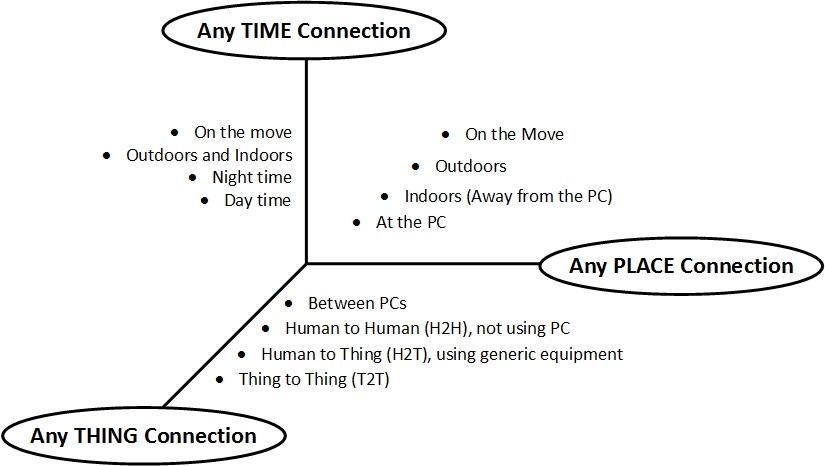
\includegraphics[scale=0.55]{./gfx/dimension}
	\centering
	\caption{\acs{IoT} Dimensions \cite{IOTFUTURE}}
	\label{fig:2.6}
\end{figure}
\subsection{Definition and Trends}
Xia et al. \cite{IOTXIA} puts forward a general \acs{IoT} definition in their editorial.
\begin{definition}
\textit{\acs{IoT}} refers to the networked interconnection of everyday objects, which are often equipped with ubiquitous intelligence. IoT will increase the ubiquity of the Internet by integrating every object for interaction via embedded systems, which leads to a highly distributed network of devices communicating with human beings as well as other devices.
\end{definition}
Gubbi et al. \cite{IOTGUBBI} explains \acs{IoT} from the point of view of the Cloud applications.
\begin{definition}
	\textit{\acs{IoT}} means interconnection of sensing and actuating devices providing the ability to share information across platforms through a unified framework, developing a Common Operating Picture (\acs{COP}) for enabling innovative applications, that is achieved by seamless ubiquitous sensing, data analytics and information representation with Cloud computing as the unifying framework.
\end{definition}
Considering the functionality and identity as central Tan et al. \cite{IOTFUTURE} defines \acs{IoT} as a new dimension that has been added to the world of \acs{ICT}: from any \textit{Time}, any \textit{Place} connectivity for anyone to now connectivity for any \textit{Thing} as shown in \reffig{fig:2.6}.
\begin{definition}
\textit{\acs{IoT}}s have identities and virtual personalities operating in smart spaces using intelligent interfaces to connect and communicate within social, environment, and user contexts.
\end{definition}
Similarly the Cluster of European Research Projects \cite{IOTEUR} explains Internet of Things as stated below.
\begin{definition}
	\textit{Things} are active participants in business, information and social processes where they are enabled to interact and communicate among themselves and with the environment by exchanging data and information sensed about the environment, while reacting autonomously to the real/physical world events and influencing it by running processes that trigger actions and create services with or without direct human intervention.
\end{definition}
\begin{figure}[h!]
	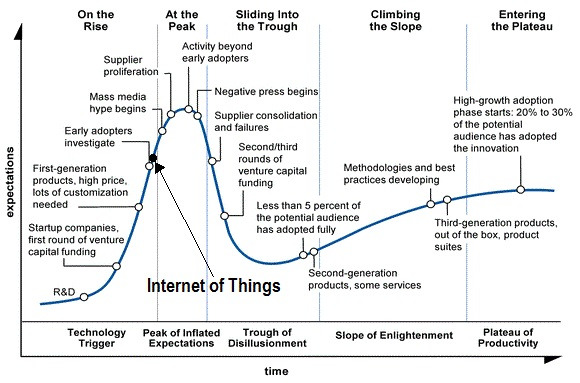
\includegraphics[scale=0.8]{./gfx/hypecycle}
	\centering
	\caption{\acs{IoT} in Gartner Hype-Cycle - Adapted from \cite{PICHYPECYC,HYPECYCGARTNER}}
	\label{fig:2.7}
\end{figure}

A \textit{Hype Cycle} is a way to represent the emergence, adoption, maturity, and impact on applications of specific technologies \cite{HYPECYCGARTNER}. \acs{IoT} has been identified as one of the emerging technologies in \acs{IT} as noted in Gartner’s \acs{IT} Hype Cycle - 2015 already shown in \reffig{fig:2.7}.  As per its estimation \acs{IoT} will take 5–10 years for market adoption. \acs{IoT} is opening tremendous opportunities for a large number of novel applications that promise to improve the quality of our lives. In recent years, \acs{IoT} has gained much attention from researchers and practitioners from around the world \cite{HYPECYCGARTNER,IOTXIA}.
\subsection{Elements of Internet of Things}
\acs{IoT} is a technological revolution that represents the future of \acs{ICT}. There are three \acs{IoT} components which enables seamless ubiquitous computing: (a) \textit{Hardware} made up of sensors, actuators and embedded communication hardware (b) \textit{Middleware} like on demand storage and computing tools for data analytics and (c) \textit{Presentation} for easy to understand visualization and interpretation tools which can be widely accessed on different platforms. Here we discuss a few enabling technologies which will make up components stated above. Things can be connected wired or wireless. In the \acs{IoT} wireless connection will to be the main way \cite{IOTGUBBI,IOTFUTURE}. Base on the existed infrastructure, there are many ways to connect a thing: Radio Frequency Identification (\acs{RFID}), Wireless Sensor Network (\acs{WSN}), Digital Subscriber Line (\acs{DSL}), General Packet Radio Service (\acs{GPRS}), WiFi, 3G Universal Mobile Telecommunications System (\acs{UMTS}), 4G Long-Term Evolution (\acs{LTE}) etc.
\subsubsection{Radio Frequency Identification}
Radio Frequency Identification (\acs{RFID}) is a non-contact technology that identifies objects attached with tags that help in the automatic identification of anything they are attached to. Sometimes \acs{RFID} has been labeled as a replacement of bar code, but \acs{RFID} system can do much more than that \cite{RFIDMIS,IOTFUTURE}.

\acs{RFID} tags consist of a $\mu$Controller, an antenna (either wire or printed using conductive carbon ink), and polymer-encapsulating material that wraps around the antenna and the chip. Readers interrogate tags for their contents through antenna and interface to back-end databases for more functionalities. \acs{RFID} can also identify mobile objects of high speed and it can identify certain amount of Tags simultaneously by its anti-collision mechanism \cite{RFIDMIS}. In addition to identify items it also can track items in real-time to get important information about their location and status \cite{IOTFUTURE}. 

The passive \acs{RFID} tags don't have  own power source and they use the power of the reader’s interrogation signal to communicate the tag to the \acs{RFID} reader. This has resulted in many applications particularly in retail, supply chain management and access control applications as well. The passive tags are currently being used in many bank cards and road toll tags which are among the first global deployments. Many
manufacturing enterprises, are taking advanced technologies to ensure its ordered and correct product procedures. Active \acs{RFID} readers have their own power source and can instantiate the communication. Major application of active \acs{RFID} tags is in port containers for monitoring cargo \cite{IOTGUBBI,RFIDMIS}.

Nanotechnology and miniaturization can make embedded intelligence in things themselves which called smart devices. They can process information, self-configure, make decision independently, just until then there will be a real \textit{thing to thing} \reffig{fig:2.6} communication \cite{IOTFUTURE}.
\subsubsection{Wireless Sensor Network}
Recent advances in {Micro-Electro-Mechanical Systems (\acs{MEMS}) technology, wireless communications, and digital electronics have enabled the development of low-cost, low-power, multi-functional sensor nodes which consist of sensing, data processing, and communicating components, leverage the idea of Wireless Sensor Network (\acs{WSN}) \cite{WSNSURVEY,BPMN4WSN}. The components that make up the WSN monitoring network include:
\begin{itemize}
	\item \textit{\acs{WSN} Hardware}: A typical \acs{WSN} node contains sensor interfaces, processing units, transceiver units and power supply \cite{IOTGUBBI}.
	\item \textit{\acs{WSN} Communication Stack}: The nodes are expected to be deployed
	in an ad-hoc manner for most applications in an appropriate topology. Nodes in a \acs{WSN} need to communicate among themselves to transmit data in single or multi-hop to a base station. Node drop outs, and consequent degraded network lifetimes, are pretty frequent \cite{IOTGUBBI,WSNSURVEY}.
	\item \textit{\acs{WSN} Middleware}: Middleware is a software layer that stands between the networked operating system and the application and provides well known reusable solutions to frequently encountered problems like heterogeneity, interoperability, security and dependability \cite{MIDDLEWARE}. Middleware such as Open Sensor Web Architecture (\acs{OSWA}) are required to provide a mechanism to combine cyber infrastructure with Service Oriented Architecture (\acs{SOA}) and sensor networks to provide access to heterogeneous sensor resources in a deployment independent manner \cite{IOTGUBBI}.
	\item \textit{Secure Data Aggregation}: An efficient and secure data aggregation method is required for extending the lifetime of the network as well as ensuring reliable data collected from sensors. Node failures are a common characteristic of \acs{WSN}, the network topology should have the capability to heal itself. Ensuring security is critical as the system is automatically linked to actuators and protecting the systems from intruders becomes very important \cite{IOTGUBBI}.
\end{itemize}
Some of the application areas of \acs{WSN} are health, military, and security. For example, a node in a \acs{WSN} might measure temperature values in a room while another node controls the air conditioning according to the sensed values and desired overall room temperature. \acs{WSN} is a part of an enterprise context now, such as monitoring and optimizing energy consumption of buildings or enabling predictive maintenance of assets \cite{BPMN4WSN,WSNSURVEY}.
\subsubsection{Addressing Schemes}
The ability to uniquely identify \textit{Things} is critical as it will allow us to uniquely identify and control billions of devices remotely through the Internet. The few most critical features of creating a unique address are: uniqueness, reliability, persistence and scalability. The Uniform Resource Name (\acs{URN}) can create replicas of the resources that can be accessed through the Uniform Resource Locator (\acs{URL}). Internet Protocol version 6 (\acs{IPv6}) also gives a very good option to access the resources uniquely and remotely. Development of a lightweight \acs{IPv6} will make addressing home appliances uniquely feasible \cite{IOTGUBBI}. 

As Gubbi et al. mentions \cite{IOTGUBBI}, \acs{WSN} cannot possess \acs{IPv6} stack to address individually and hence a subnet with a gateway having a \acs{URN} will be required. At the subnet level, the \acs{URN} for the sensor devices could be the unique IDs rather than human-friendly names as in the \acs{WWW}, and a lookup table at the gateway to address this device. Further, at the node level each sensor will have a \acs{URN} (as numbers) for sensors to be addressed by the gateway. The entire network now forms a web of connectivity from users (high-level) to sensors (low-level) that is addressable through \acs{URN}, accessible through \acs{URL} and controllable through Uniform Resource Citation (\acs{URC}) \cite{IOTGUBBI}.

\subsubsection{Storage and Analytics}
The data gathered from \acs{IoT} devices have to be stored and used intelligently for smart monitoring and actuation. State-of-the-art non-linear, temporal machine learning methods based on evolutionary algorithms, genetic algorithms, neural networks, and other artificial intelligence techniques are necessary to achieve automated decision making. Cloud based storage solutions are becoming increasingly popular and in the years ahead, Cloud based analytics and visualization platforms are foreseen, since a centralized infrastructure to support storage and analytics is the most important need of the hour \cite{IOTGUBBI}.

\subsubsection{Visualization}
Visualization is critical for an \acs{IoT} application as this allows the interaction of the user with the environment. It enables policy makers to convert data into knowledge, which is critical in fast decision making. Extraction of meaningful information from raw data is non-trivial. This encompasses both event detection and visualization of the associated raw and modeled data, with information represented according to the needs of the end-user \cite{IOTGUBBI}.

\subsection{Internet of Things Architecture}
\acs{IoT} is not a theory, it's an application technology which our life can benefit from. Current Internet has a five-layered \acs{TCP}/\acs{IP} architecture, which has worked well for a long time. However, in the \acs{IoT} billions of objects are connected which will create much larger traffic and need much more data storages \cite{IOTFUTURE}. The vision of \acs{IoT} can be seen from two perspectives - ‘Internet’ centric and ‘Thing’ centric. The Internet centric architecture will involve internet services being the main focus while data is contributed by the objects. In the object centric architecture, the smart objects take the center stage \cite{IOTGUBBI}. Tan et al. \cite{IOTFUTURE} proposed an Internet-centric approach in their work.
\begin{figure}[h!]
	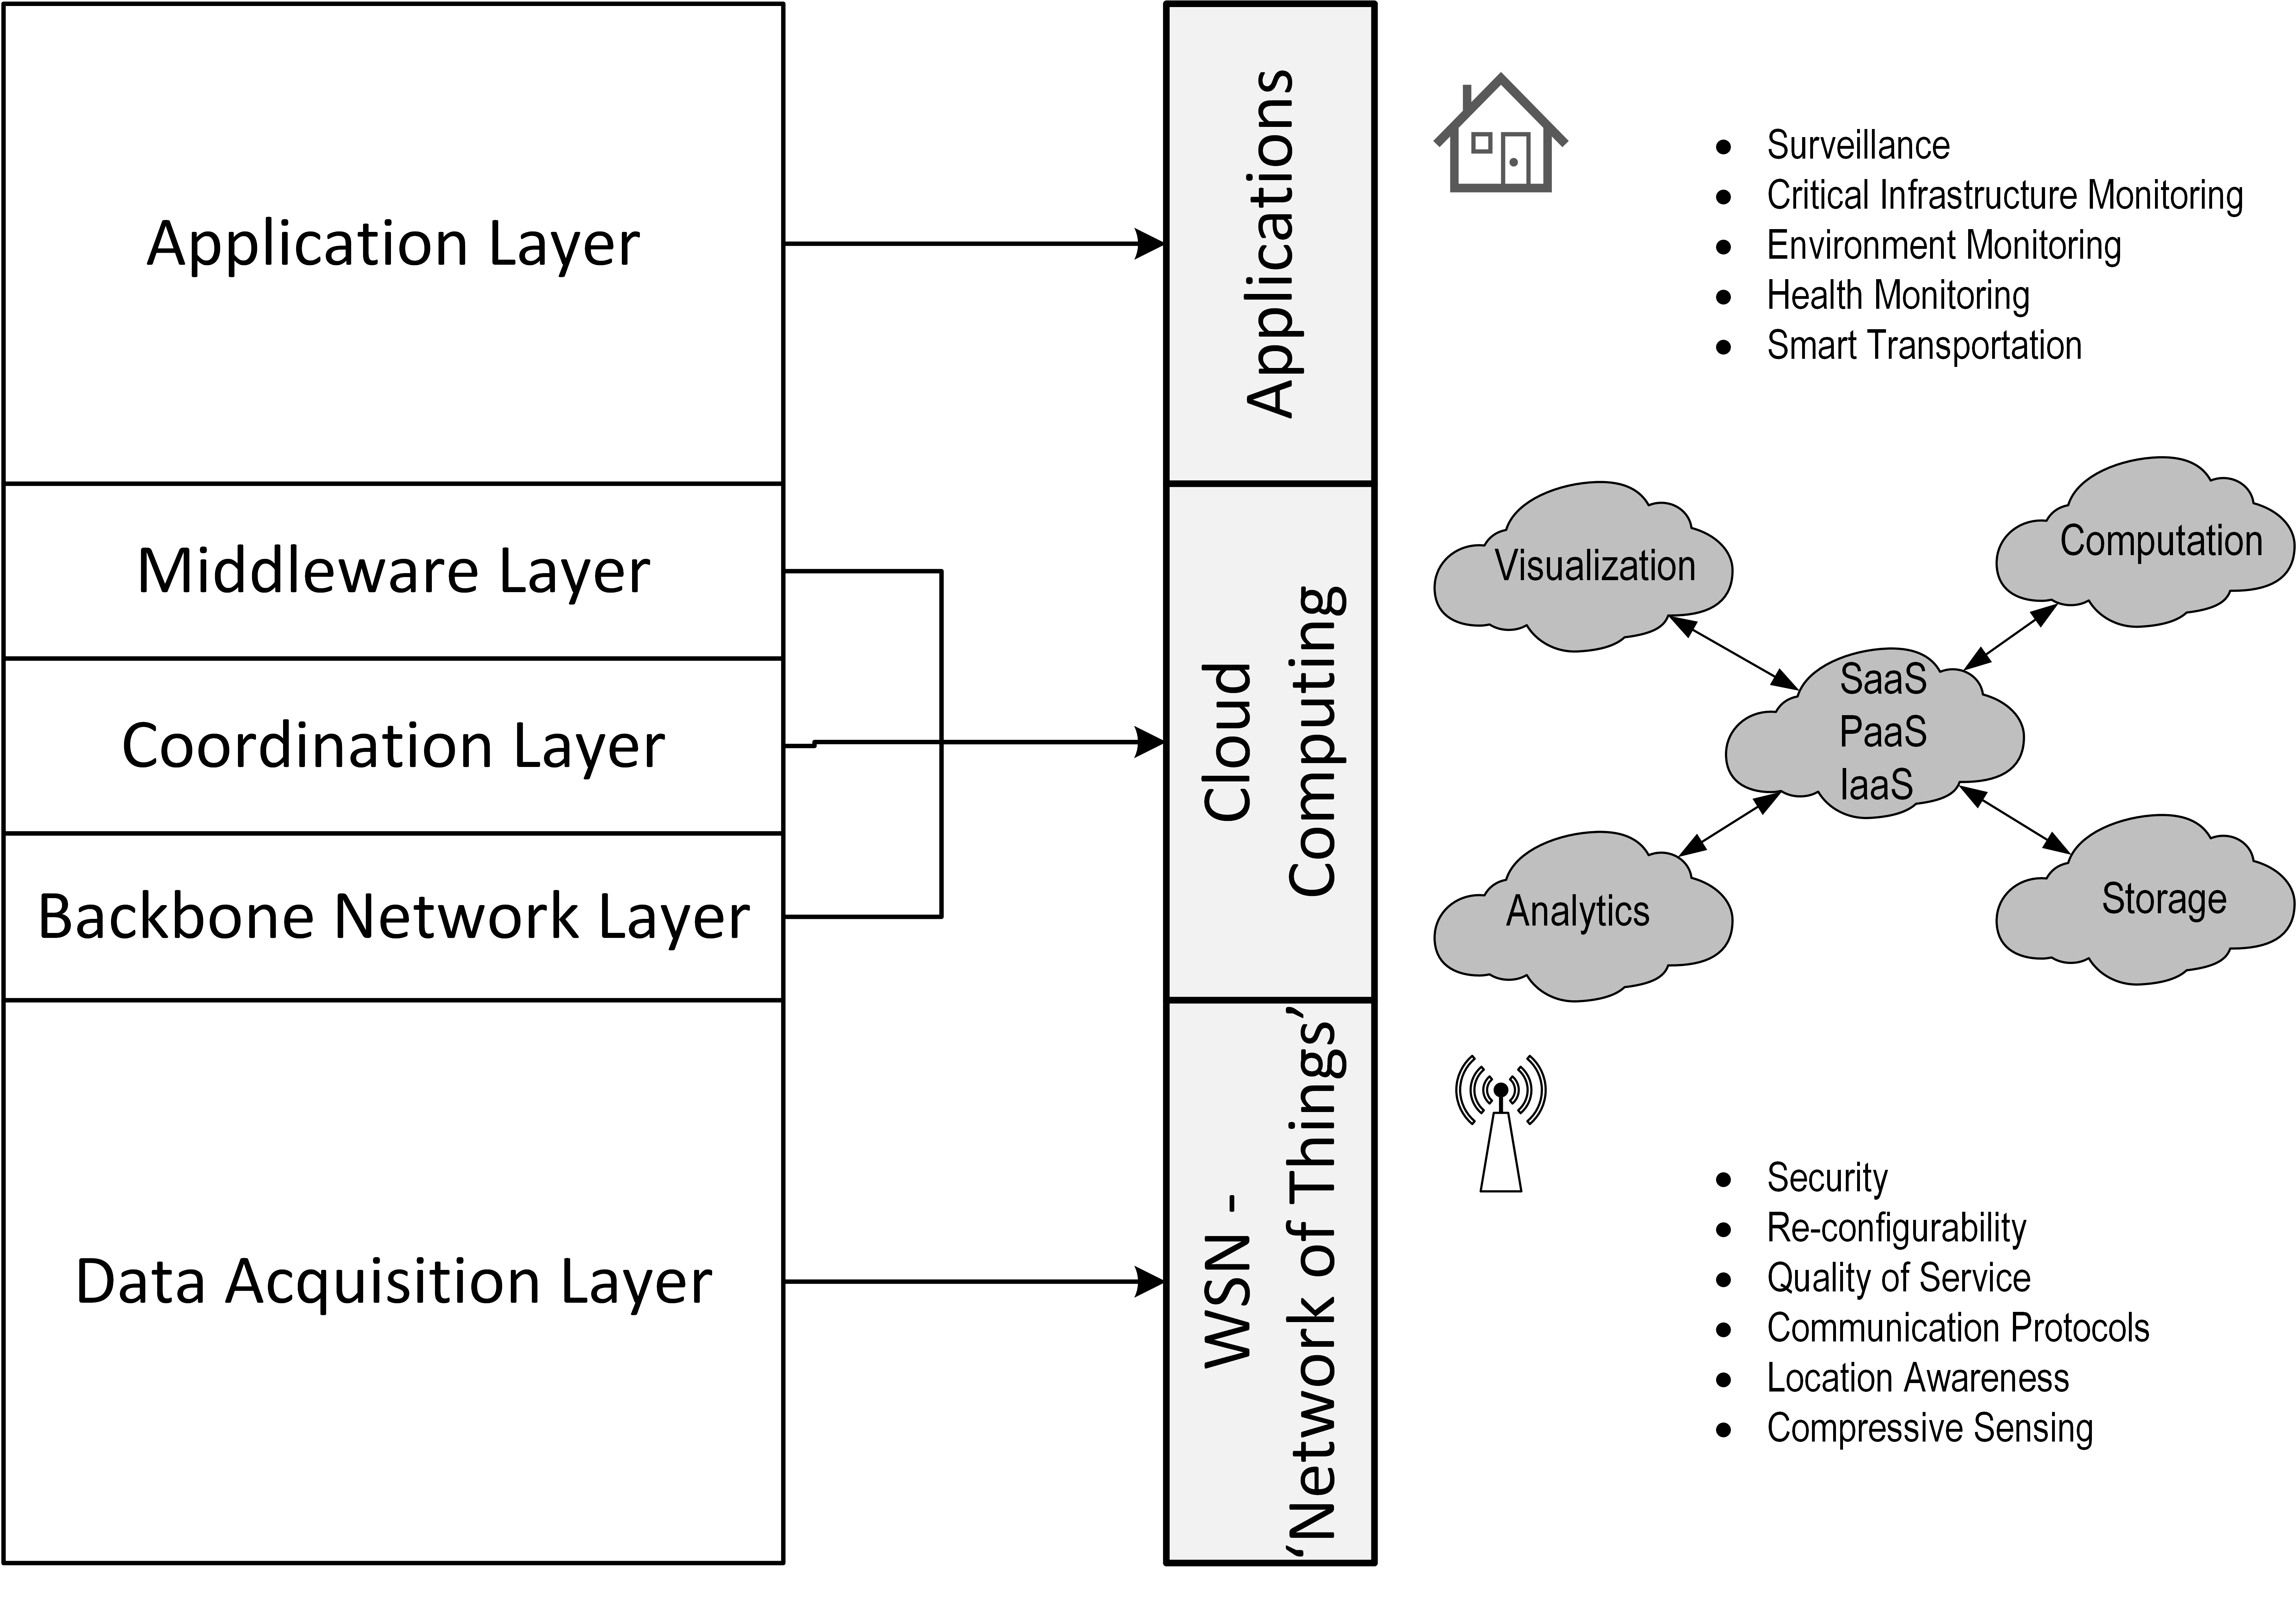
\includegraphics[scale=0.5]{./gfx/iotarch}
	\centering
	\caption{Conceptual \acs{IoT} Architectural Framework - Adapted from \cite{IOTFUTURE,IOTGUBBI}}
	\label{fig:2.8}
\end{figure}

A simpler conceptual framework out of architecture proposed by Tao et al. \cite{IOTFUTURE} integrating the ubiquitous sensing devices and the applications is proposed by us which is shown in \reffig{fig:2.8} \footnote{\acs{IaaS} = Infrastructure as a Service\\\acs{PaaS} = Platform as a Service\\\acs{SaaS} = Software as a Service}. In order to realize the full potential of cloud computing as well as ubiquitous sensing, a combined framework with a cloud at the center seems to be most viable \cite{IOTGUBBI}. 

The \textit{Backbone Network Layer} may be today's Internet, may be not or may be its expansion. The \textit{Coordination Layer} responses to process the structure of packages from different application systems and reassemble them to an unified structure which can be identified and processed by every application system to make it inter-operable among the already existing systems and the newly deployed systems \cite{IOTFUTURE}. As per our evaluation of the model, the three layers in the middle (Middleware, Coordination and Backbone Network) of Tao et al. \cite{IOTFUTURE} can be integrated and realized as a single layer of Cloud Computing as proposed by Gubbi et al. \cite{IOTGUBBI}.

According to Perera et al. \cite{CONAWAREIOT} \acs{IoT} should be facilitated by a hybrid architecture which comprises primarily two different architectural approaches, namely event driven and time driven. Some sensors produce data when an event occurs (e.g. door sensor); the rest produce data continuously, based on specified time frames (e.g. temperature sensor)  \cite{CONAWAREIOT}.

Sensing service providers can join the network and offer their data using a storage cloud; analytic tool developers can provide their software tools; artificial intelligence experts can provide their data mining and machine learning tools useful in converting information to knowledge and finally computer graphics designers can offer a variety of visualization tools. Cloud computing can offer these services as Infrastructures, Platforms or Software where the full potential of human creativity can be tapped using them as services \cite{IOTGUBBI}. 

\subsection{Cyber-Physical Systems} \label{CPS}
Cyber-Physical Systems (\acs{CPS}) are integrated automated systems that enable connection of the operations of the physical reality with computing and communication infrastructures. \acs{CPS} goes with the trend of having information and services everywhere at hand, and it is inevitable in the highly networked world of today. Fields of applications for \acs{CPS} include medical equipment, driving safety and driver assistance systems for automobiles, industrial process control and automation systems, assistance systems for controlling the power supply in terms of optimized use of renewable energies \cite{CYBERIN,IN4DESIGN}. 

A \acs{CPS} consists of a control unit, usually one or more $\mu$Controller(s), which control(s) the sensors and actuators that are necessary to interact with the real world, and processes the data obtained \reffig{fig:2.9}. \acs{CPS} also requires a communication interface to exchange data with other \acs{CPS} or a cloud. In other words, a \acs{CPS} is an embedded system that is able to send and receive data over a network. The \acs{CPS} connected to the Internet is often loosely referred to as the \acs{IoT} \cite{CYBERIN}. 
\begin{figure}[h!]
	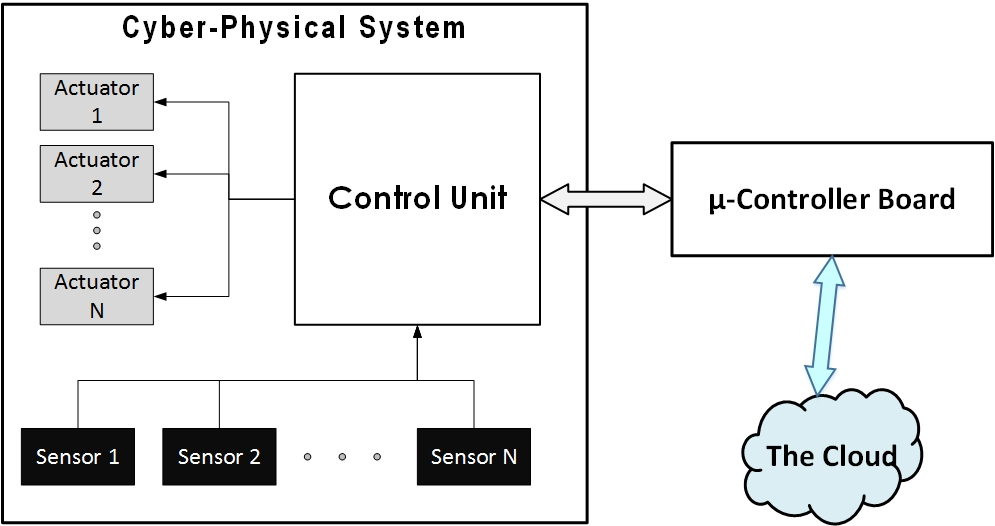
\includegraphics[scale=0.5]{./gfx/cpsdiag}
	\centering
	\caption{Conceptual Architecture of a \acs{CPS} - Adapted from \cite{CYBERIN}}
	\label{fig:2.9}
\end{figure}

The development of \acs{CPS} is characterized by three phases. The first generation of \acs{CPS} includes identification technologies like \acs{RFID} tags, where storage and analytics have to be provided as a centralized service. The second generation of \acs{CPS} are equipped with sensors and actuators with a limited range of functions. \acs{CPS} of the third generation can store and analyze data, are equipped with multiple sensors and actuators, and are network compatible \cite{IN4DESIGN}. To sum it up, a \acs{CPS} requires three levels as pointed out by Drath et al. \cite{IN4HYPE}:
\begin{itemize}
	\item the physical objects,
	\item data models of the mentioned physical objects in a network infrastructure, and
	\item services based on the available data.
\end{itemize}
Due to the rise of \acs{CPS} components, products, and other entities in industrial production would get their own identities in the network such that hey could be interconnected and simulated. Systems could be virtually integrated, tested, and optimized. The digital factory and the virtual commissioning would be accessible
to everybody. Products could navigate autonomously through the production line. This will establish \acs{CPS} as one of the the prime enablers of Industry 4.0 - the forthcoming industrial revolution \cite{IN4HYPE,IN4BCG}.
\subsection{Smart Factory and Industry 4.0} \label{smartfactory}
In manufacturing, there is great potential for \acs{CPS} to improve the production process and the supply chain. The \acs{IoT} has set in motion Industry 4.0 will disperse control. Consider processes that govern themselves, where smart products can take corrective action to avoid damages and where individual parts are automatically replenished. Such technologies already exist and could drive Industry 4.0 further. As suggested by Siegfried Dais in a conversation with L{\"o}ffler et al. \cite{IOTMANU}, two competencies must come together to drive development further: using what’s truly new about new technologies and finding hum an resource who can design robust algorithms to make the system user-friendly and robust. The trend of separating design and production will continue to spread across other industries and sectors. Likewise, supply-chain integration will play a decisive role in new operating models \cite{IOTMANU}.

Lean Production principles are widely accepted in industry which refers to the strict integration of humans in the production process, a continuous improvement and focus on value adding activities by avoiding of waste. If a plant implements lean manufacturing, it keeps its stocks to a minimum - neither one part too many nor too few. With the \acs{IoT}, this system must extend beyond the limits of individual factories to interconnect multiple factories and even regions. Instruments to reach this increased automation are \acs{CPS}. \acs{CPS} can work autonomously and interact with their production environment. As a result, a factory becomes \textbf{\textit{‘Smart Factory’}} \cite{LEANKOLBERG,IOTMANU}.

The department of \acs{IFS} at the German Research Center for Artificial Intelligence (\acs{DFKI}) identified four enablers as shown in \reffig{fig:2.10} for the \textit{Smart Factory} \cite{LEANKOLBERG}: 
\begin{itemize}
	\item \textit{Smart Operator}: People can supervise and control ongoing activities in ease e.g. equipped with smart watches, employees receive error messages and error locations close to real time. \acs{CPS} equipped with proper sensors can recognize failures and automatically trigger fault-repair actions on other \acs{CPS}. \cite{LEANKOLBERG}.
	\item \textit{Smart Product}: It could collect process data for the analysis during and after its production. In contrast to manual data acquisition for value stream mapping it is possible to gather information individualized per product and production line automatically. This way of data acquisition is less labor-intensive and data are more precise \cite{LEANKOLBERG}.
	\item \textit{Smart Machine}: Especially the potential of \acs{CPS} in production is not fully explored yet. Machines help employees to avoid mistakes. With their computing capacity and connectible sensors, \acs{CPS} could be integrated fast and flexible in fault-prone processes for supporting \cite{LEANKOLBERG}.
	\item \textit{Smart Planner}: It could optimize processes in real-time. \acs{CPS} could supports optimization of production processes by different business objectives, like throughput time or efficacy. Applied to Lean Production, this approach could enable Lean Production to be implemented not only in mass and batch production, but also in job shop production \cite{LEANKOLBERG}.
\end{itemize}

In the context of Industry 4.0 new solutions are available for combining automation technology with Lean Production. As described above, the combination of automation technology and Lean Production can be beneficial. Contrary to popular belief, Lean Production does not exclude automation \cite{LEANKOLBERG}. It is essential to translate the physical world into a format that can be handled by \acs{IT} which requires mathematical, domain, market, and domain know-how. 

As suggested by Heinz Derenbach in a conversation with L{\"o}ffler et al. \cite{IOTMANU}, separating the physical world from business processes will be a foolish idea. It means a physical device or \textit{'Things'} becomes an active part of a business process: delivering data, sending events, and processing rules. This notion is driving manufacturing sector and Industry 4.0. The next big step will be to think through the interdependencies among the machine, the production components, the manufacturing environment, and the \acs{IT} that connects it all. This requires a high degree of standardization so that the machine knows what it needs to do to any given component, and the components can confirm that the machine has done it. Such \acs{IT} linkage goes far beyond current manufacturing systems \cite{IOTMANU}.
\begin{figure}[h!]
	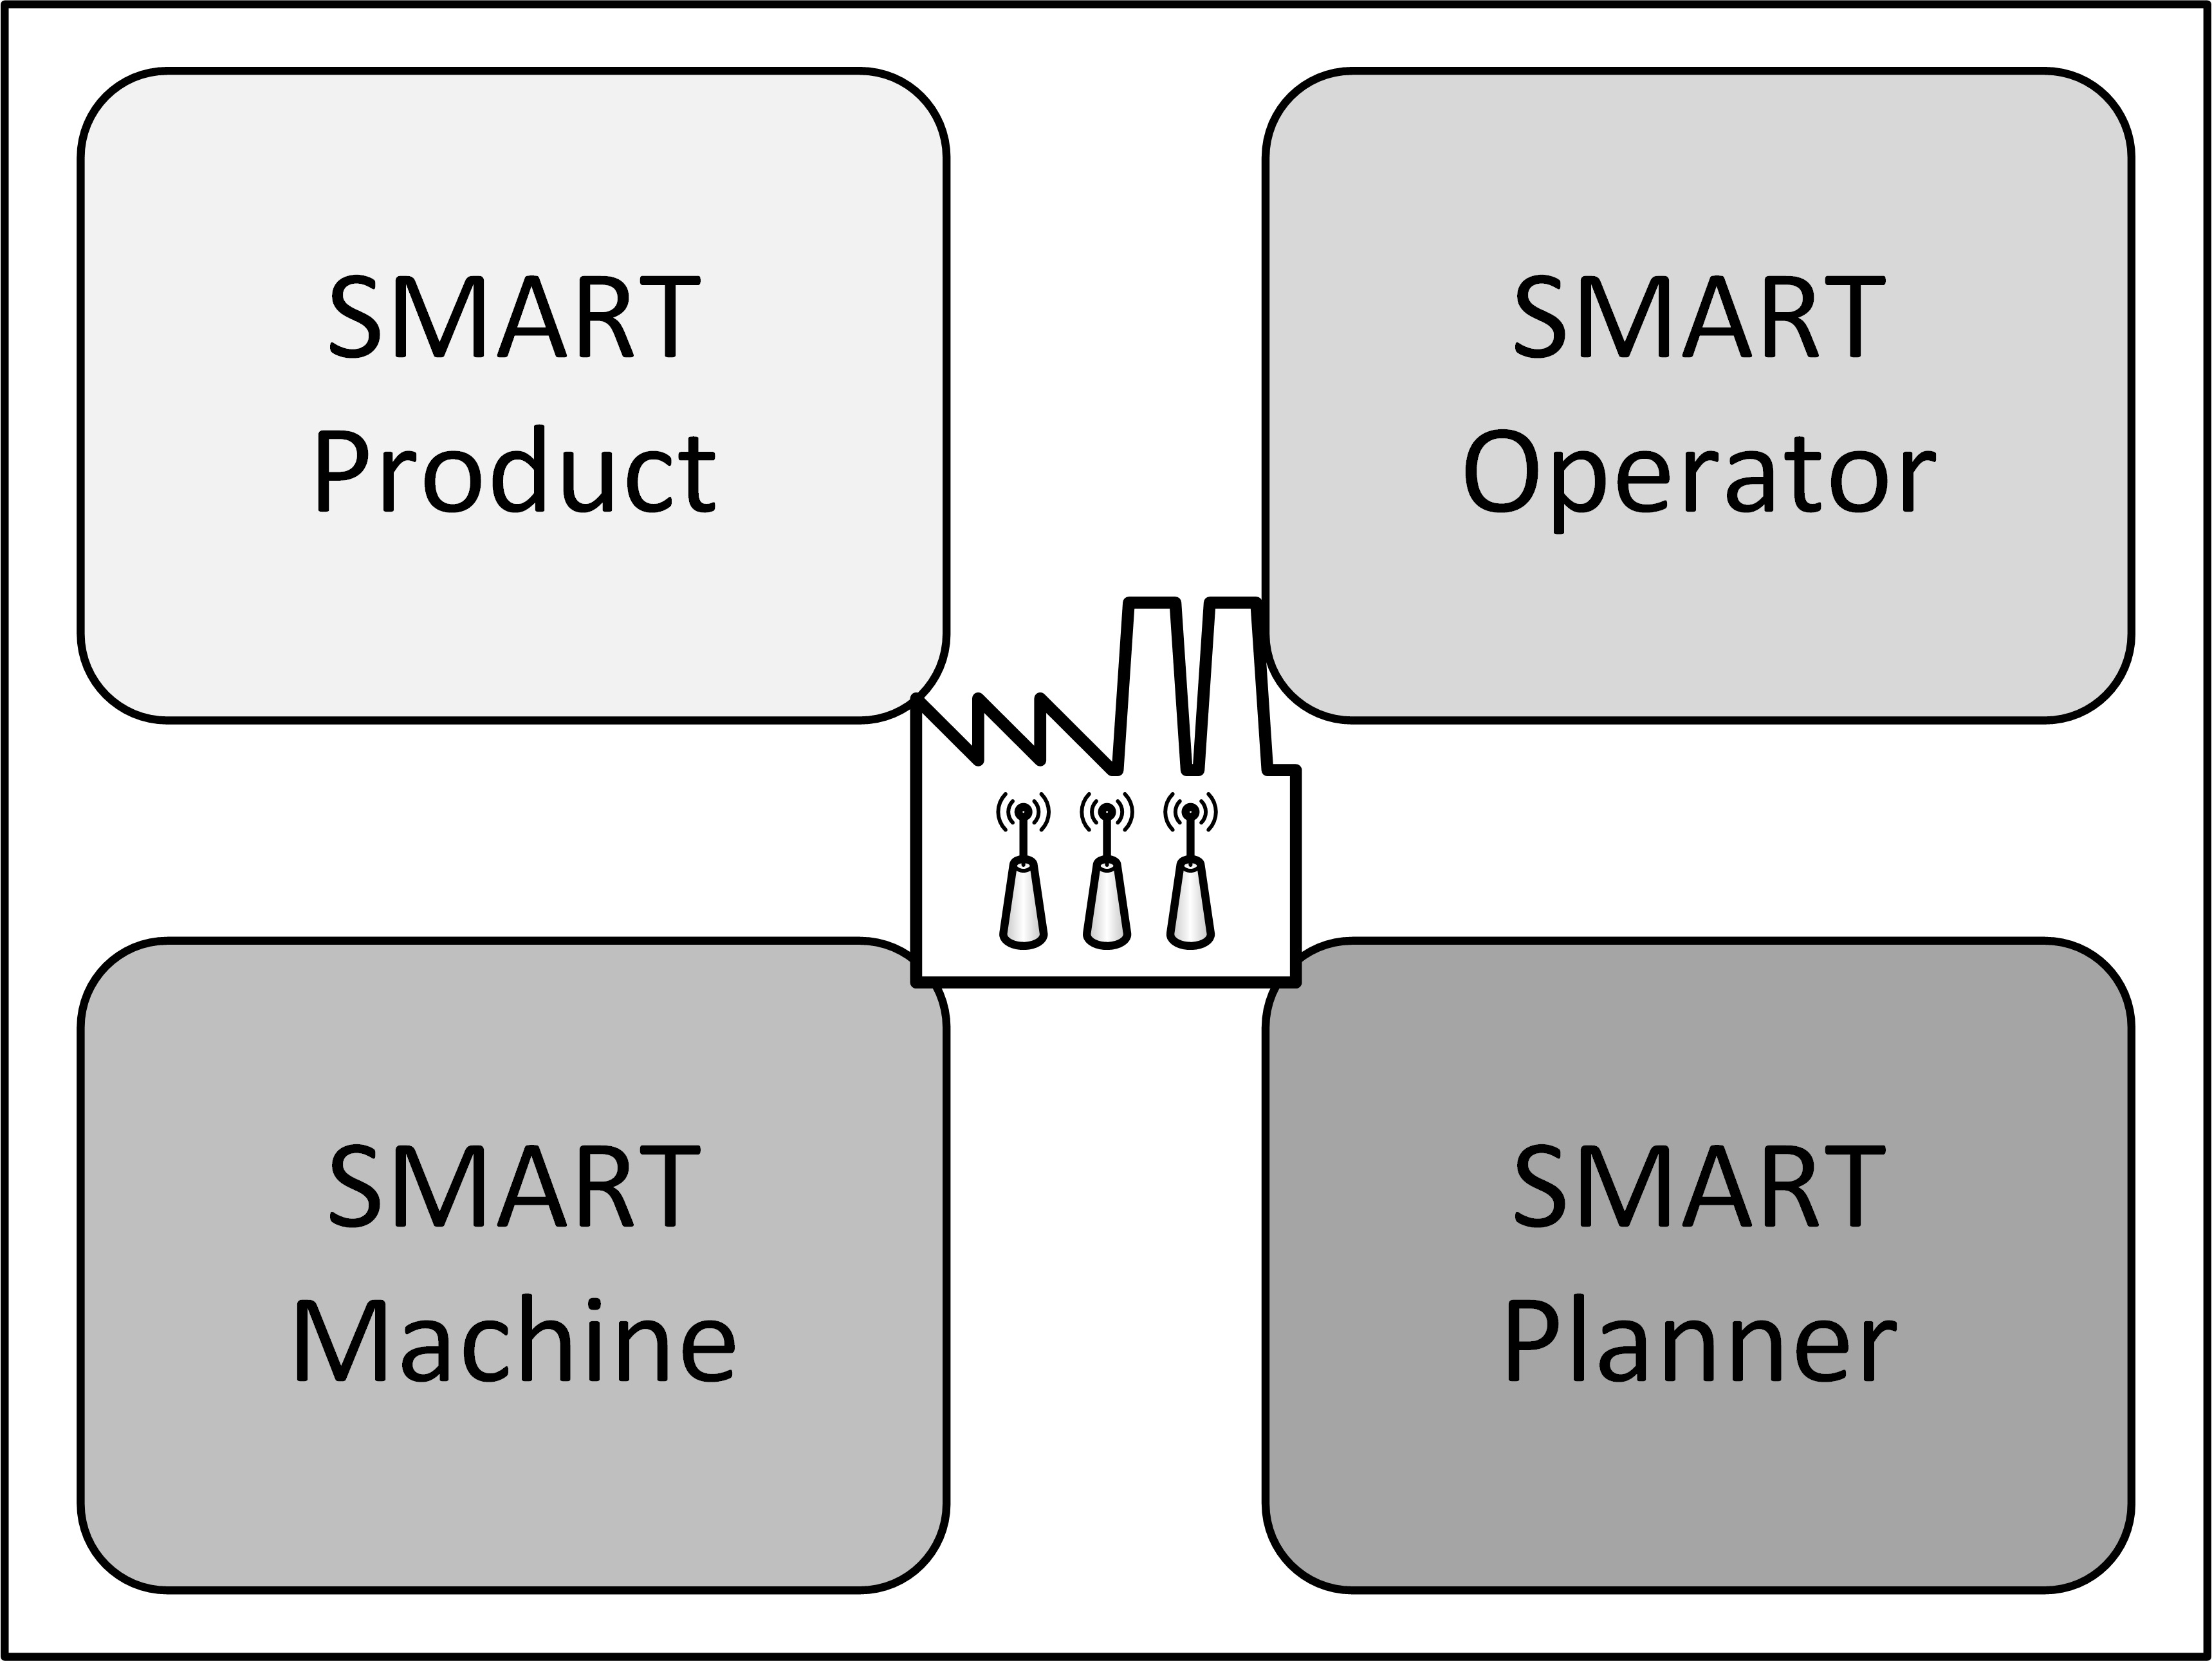
\includegraphics[scale=0.6]{./gfx/smartfac}
	\centering
	\caption{Enablers of Smart Factory}
	\label{fig:2.10}
\end{figure}
Due to the exponentially increasing amount of data and knowledge relevant for manufacturing planning and optimization, it is impossible for one or a team of production engineers to have all these information in mind. Therefore we search for a possibility to support manufacturing planning and optimization activities by enhancing digital tools with \acs{IoT} enabled \acs{CPS}. This is of a very interdisciplinary character. On the one hand there is the need for a detailed understanding of the production process being planned, based on knowledge and experiences of experts in the field of manufacturing engineering that usually have limited interest in \acs{ICT}. On the other hand, the handling of this large amount and high complexity of information is a challenging task for \acs{IT} experts who in turn do not have complete knowledge of the production processes \cite{LANDHERR}. 

Still \acs{IoT} technology has a wide range of applications in many fields, including aerospace, automotive, communication, medical and, manufacturing industry, and so on. For example, in the field of aerospace industry, the application of \acs{IoT} can effectively improve the product’s safety and reliability by identifying the fake and shoddy parts or products. In the automotive industry, IoT is widely used in the production line, quality monitor and control, assemble line, logistics and product (or part) tracking, and the real-time link of customer service. Among the procedure, intelligent labels are posted on the components in every part of the link to make it easy to track or invoke, together with the associated attribute information, such as the manufacturer’s name, serial number, product type, product code, the place and time of the production, as well as the exact location of the product \cite{IOTCLOUD,CONAWAREIOT}.

\subsection{Challenges Ahead for Internet of Things} \label{smartfactory}
The \acs{IoT} is the wheel of Industry 4.0, but there are many issues need to be addressed. In this part we discuss three crucial issues among many issues such as, standardization, security and privacy, and energy efficiency \cite{IOTFUTURE,IOTGUBBI}.

There can be no real \acs{IoT} without a global standard. But the fact is technological standardization of the \acs{IoT} in most areas is still in its infancy, or remain fragmented. So efforts are needed, collaboration among International Organization for Standardization (\acs{ISO}), European Telecommunications Standards Institute (\acs{ETSI}), Internet Engineering Task Force (\acs{IETF}), International Telecommunication Union (\acs{ITU}), Institute of Electrical and Electronics Engineers (\acs{IEEE}) and other related organizations is very important and urgent. As the \acs{WWW} grew in last decade, many security and privacy problems came out, then we could do nothing but build patches and it seems that the security and privacy is an add-on feature. But the public acceptance for the \acs{IoT} will happen only when the strong security and privacy solutions are in place. So we should take security and privacy a very important role from the early design and build phase in the \acs{IoT} \cite{IOTFUTURE}. Sensor nodes carry limited, generally irreplaceable, power sources. Therefore, while traditional networks aim to achieve high \acs{QoS} provisions, sensor network protocols must focus primarily on power conservation. They must have inbuilt trade-off mechanisms that give the end user the option of prolonging network lifetime at the cost of lower throughput or higher transmission delay \cite{WSNSURVEY}.

Manufacturing industry can benefit immensely from the \acs{IoT}. Though the future is bright, there still are many technical issues need to be addressed and a long path to realize \acs{IoT}. As per L{\"o}ffler et al. \cite{IOTMANU}, "Process and Device" will be inseparable; physical things become part of the process. Machines and workflows will merge to become a single entity. \acs{IoT} activities are gathering momentum around the world, with numerous initiatives underway across industry, academia and government, as key stakeholders seek to map a way forward for the coordinated realization of this evolution towards Industry 4.0 \cite{IOTFUTURE,IOTGUBBI,IOTMANU}.

\chapter{Context-sensitive Workflows}  \label{conces}
%Context-aware applications adapt their behavior based on changes of the physical world, which is often obtained with a huge amount of sensors. Thus, the development of such applications is cumbersome, in particular the implementation of their often complex control flow. To ease the development of context-aware applications we present the concept of context-aware workflows. Thereafter we present an implementation of these concepts based on a standard workflow language. Context-aware workflows are not only interesting for the development of context-aware applications, but also enable workflow technology to be applied in new domains that are process oriented and yet not supported by workflow systems like production processes in the manufacturing industry. The concept of context-aware workflows is a first approach that enables modeling and execution of technical production processes with workflow systems normally used for business processes.
%\subsection{Definitions}
%\begin{figure}[h!]
%	\includegraphics[scale=0.62]{./gfx/myarch}
%	\centering
%	\caption{Enablers of Smart Factory}
%	\label{fig:2.10}
%\end{figure}
\subsection{Proposed System}
\subsection{Operational Semantics}
\subsection{Realization Architecture}
